\documentclass{report}

\usepackage{mathtools}
\usepackage{amsmath}
\usepackage{amsfonts}
\usepackage{amsthm}
\usepackage{amssymb}

\theoremstyle{plain}
\newtheorem{thm}{Theorem}
\newtheorem{lem}[thm]{Lemma}
\newtheorem{prop}[thm]{Proposition}
\newtheorem*{cor}{Corollary}

\theoremstyle{definition}
\newtheorem{defn}{Definition}
\newtheorem{conj}{Conjecture}
\newtheorem{exmp}{Example}

\theoremstyle{remark}
\newtheorem*{rem}{Remark}

\usepackage{systeme}

\usepackage[T1]{fontenc}
\usepackage{dsfont}

\usepackage[top=2.5cm, left=3cm, right=3cm, bottom=2.5cm]{geometry}
\usepackage[demo]{graphicx}
\usepackage{caption}
\usepackage{subcaption}

\usepackage{etoolbox}
\listadd{\pc}{$C$}
\listadd{\pc}{$C\sharp$}
\listadd{\pc}{$D$}
\listadd{\pc}{$E\flat$}
\listadd{\pc}{$E$}
\listadd{\pc}{$F$}
\listadd{\pc}{$F\sharp$}
\listadd{\pc}{$G$}
\listadd{\pc}{$G\sharp$}
\listadd{\pc}{$A$}
\listadd{\pc}{$B\flat$}
\listadd{\pc}{$B$}
\listadd{\pcs}{$B$}
\listadd{\pcs}{$C$}
\listadd{\pcs}{$C\sharp$}
\listadd{\pcs}{$D$}
\listadd{\pcs}{$E\flat$}
\listadd{\pcs}{$E$}
\listadd{\pcs}{$F$}
\listadd{\pcs}{$F\sharp$}
\listadd{\pcs}{$G$}
\listadd{\pcs}{$G\sharp$}
\listadd{\pcs}{$A$}
\listadd{\pcs}{$B\flat$}

\usepackage{calc}

%\usepackage[pageanchor]{hyperref}
\captionsetup{margin=10pt,font=small,labelfont=bf}

\usepackage{tikz}
\usetikzlibrary{arrows,decorations.markings}
\usetikzlibrary{cd}
\usetikzlibrary{shapes.geometric,fit}
\usetikzlibrary{positioning}
\usepackage{floatrow}

\newenvironment{tzfigure}[1]
{
    \begin{figure}[ht]
        \centering
        #1
        \begin{tikzpicture}
}
{
        \end{tikzpicture}   
    \end{figure}
}

\newenvironment{tzcategory}[1]
{
    \begin{figure}[ht]
        \centering
        #1
        \begin{tikzpicture}[baseline= (a).base]    
}
{
    \end{tikzpicture}   
\end{figure}
}

\newenvironment{subtzcategory}[2]
{
    \begin{subfigure}[ht]{#2}
        \centering
        #1
        \begin{tikzpicture}[baseline= (a).base]    
}
{
    \end{tikzpicture}   
\end{subfigure}
}


\usepackage{ stmaryrd }
\newcommand{\prodmon}{\Pi}
\newcommand{\phieq}{\stackrel{\mathclap{\normalfont\mbox{$\phi$}}}{\cong}}

\usepackage[refpage]{nomencl}
\makeatletter
\def\nomlabelref#1{\dotfill\nobreakspace page\ \pageref{#1}\nomentryend\endgroup}
\def\@@@nomenclature[#1]#2#3#4{%
 \def\@tempa{#2}\def\@tempb{#3}\def\@tempc{#4}%
 \protected@write\@nomenclaturefile{}%
  {\string\nomenclatureentry{#1\nom@verb\@tempa @[{\nom@verb\@tempa}]%
      \begingroup\nom@verb\@tempb\protect\nomeqref{\theequation}%
        |nomlabelref}{\@tempc}}%
 \endgroup
 \@esphack}
\makeatother
\usepackage[backref=page,pageanchor]{hyperref}
\renewcommand{\nomname}{Notations}
\renewcommand{\nompreamble}{The next list describes several notations used throughout this document.}
\makenomenclature



\begin{document}

%\begingroup    

\title{Categories and music}
\author{Alice Rixte}
\date{\today}
\maketitle %\endgroup

\section*{Acknowledgement}
Je souhaite remercier du fond du cœur Carlos Agon, mon encadrant de stage, pour son ouverture d'esprit, sa joie et sa motivation communicatives et son soutien tout au long de ce stage. Mille merci à Alexandre Popoff pour ses nombreux conseils, pour le temps qu'il m'a accordé si généreusement et pour avoir créé un terrain de jeu aussi amusant que celui des PK-nets. Merci à Andrée Ehresmann pour ses conseils et ses recommendations avisées.

Merci à mon canard en plastique préféré, ma famille et mes amis, sans le soutien desquels je n'irais pas bien loin (même sans savoir vraiment où l'on va).
\nomenclature[Ii]{$I_i$}{$i^\text{th}$ inversion}{nomencl:Ii}
\nomenclature[TI]{$T/I$}{The group of transpositions and inversions acting on the set of pitch classes}{nomencl:TI}
\nomenclature[Ti]{$T_i$}{Transposition of $i$ semitones}{nomencl:Ti}
\nomenclature[Zn]{$\mathbb{Z}_n$}{The cyclic group of order $n$}{nomencl:Zn}


\tableofcontents


\chapter{Introduction}

Transformational music theory is a way to analyse music by focusing on the transformations between musical object rather than on the objects themselves. It was mainly developped by David Lewins in 1980's \cite{rahn_lewin_1987}. His work relied on algebra, and particularly on group theory. Indeed, by using well temperament, we obtain a 12 element dodecahedron, with each vertex corresponding to one of the 12 semi-tones. There are then 12 rotational symmetries and 12 axial symmetries of this dodecahedron (called  respectively \textbf{transpositions} and \textbf{inversions} and written $T_i$ and $I_i$ for $i\in [\![1,12]\!]$ by music theorists).

\newcounter{itemcount}
\setcounter{itemcount}{450}
\renewcommand*{\do}[1]{
    \filldraw [black](\number\value{itemcount}:3cm) 
    circle (1.5pt)
    node[anchor={\number\value{itemcount}-180}]
        {#1\addtocounter{itemcount}{-30}};
}
\begin{tzfigure}{
        \caption{The C Major chord in the chromatic circle}
        \label{Cmajor}
    }
    \dolistloop{\pc}
    \draw[fill=blue!20] (90:3cm) -- (330:3cm) -- (240:3cm) -- cycle;
    \draw [domain=0:360,samples=60] plot ({3*cos(\x)}, {3*sin(\x)});
\end{tzfigure}



\paragraph{Constraint in music}




\section{Presentation of Allen Forte's work}
\begin{defn}
    A \textbf{pitch class} consists of all the pitches separated with a whole number of octaves.
\end{defn}

\newcounter{itemcount}
\setcounter{itemcount}{450}
\renewcommand*{\do}[1]{
    \filldraw [black](\number\value{itemcount}:3cm) 
    circle (1.5pt)
    node[anchor={\number\value{itemcount}-180}]
        {#1\addtocounter{itemcount}{-30}};
}
\begin{tzfigure}{
        \caption{The C Major chord in the chromatic circle}
        \label{Cmajor}
    }
    \dolistloop{\pc}
    \draw[fill=blue!20] (90:3cm) -- (330:3cm) -- (240:3cm) -- cycle;
    \draw [domain=0:360,samples=60] plot ({3*cos(\x)}, {3*sin(\x)});
\end{tzfigure}

The set of all pitch classes comes naturally with a group structure, which is actually the group $\mathbb{Z}_{12}$\label{nomencl:Zn}. Indeed, we can associate $C$ to the pitch class $0$, $C\sharp$ to the pitch class $1$ and so on. We then have the possibillity to represent a $C$ major chord  from a geometrical point of vue (see \hyperref[Cmajor]{Figure \ref*{Cmajor}}).


The idea of Forte relies on the fact that a major chord will always have the same representation up to 12 rotations in this geometrical paradigm. In mathematics they are the 12 rotational symmetries of the regular dodecahedron.In music theory, these rotations are called \textbf{transpositions} and are named $T_i$\label{nomencl:Ti} for $i\in[\![0,11]\!]$.

His intuition was that instead of considering triads (three notes chord) as the set of the notes that compose them, we should consider them as the set of the intervals between each note. As a result, every inversion of chord \footnote{the term inversion has to be taken here from a musical point of view, for instance the inversions of a C major chord are C-E-G, G-C-E, E-G-C. Later in this report, we will use inversion with another definition and we will stick to it.} will be in the same \textbf{pitch-class set}\cite{forte_1980}. This can be seen in the geometrical point of view where the simple fact  of representing the chord as a triangle allow to forget any order between the three note. Similarly, all the transpositions of the chord will be in the same pitch-class.

\paragraph{Contribution (sort of)}
From another point of view, the work of Forte can be seen as networks, as in \hyperref[transpose_net]{Figure \ref*{transpose_net}}. Nonetheless, this representation does not allow for the moment to embed the notion of pitch-class set of Forte. For this we have to introduce the Klumpenhouwer networks.
\begin{tzcategory}{
        \caption{Transpositional network}
        \label{transpose_net}
    }
    \node[scale=1.3] (a) at (0,0){
        \begin{tikzcd}
            G                                                            \\
            E \arrow[u, "T_3", bend left]                                \\
            C \arrow[u, "T_4", bend left] \arrow[uu, "T_7"', bend right]
        \end{tikzcd}};
\end{tzcategory}



\section{Presentation of Klumpenhouwer's networks}
In  the 1980s, David Lewin developped a branch of music theory called transformational theory\cite{rahn_lewin_1987}. It consists of, rather than looking the musical objects for themselves but instead to mathematically study the relation between them.
%TODO read rahn_lewin_1987

Klumpenhouwer networks, or K-nets, were then introduced by Henry Klumpenhouwer, former PhD student of Lewin, to formalize the relation between two chords\cite{lewin_1990}.

We have seen that the rotations of the dodecahedron match with the notion of transposition. However, there another type of symmetry in the dodecahedron : the $12$ reflexion symmetries (see\hyperref[inversions]{Figure \ref*{inversions}}), called \textbf{inversions}\label{nomencl:Ii} in transformational music theory. Along with transposition, they form the $T/I$\label{nomencl:TI} group, otherwise known in mathematics as the \textbf{dihedral group} of a dodecahedron.

\setcounter{itemcount}{450}

\begin{tzfigure}{
        \caption{The $I_0$ inversion}
        \label{inversions}
    }
    \tikzset{myptr/.style={decoration={markings,mark=at position 1 with
                            {\arrow[scale=3,>=stealth]{>}}},postaction={decorate}}}
    \dolistloop{\pc}
    \draw [domain=0:360,samples=60] plot ({3*cos(\x)}, {3*sin(\x)});
    \draw [dashed,purple] (90:3cm) -- (270:3cm);
    \foreach \i in {1,...,5}{
            \draw [<->, >=stealth, thick, purple] (90 + \i*30:3cm) -- (90-\i*30:3cm) ;
        }
\end{tzfigure}


The idea behind K-nets is that instead of analyse chords transformations threw transposition only, which is not very rich, we could use also inversions.

\begin{defn}
    A Klumpenhouwer network is a graph (also called a network) where objects are pitch classes and arrows between objects are labeled by an element of the group $T/I$.
\end{defn}

\begin{defn}
    Two K-nets $K$ and $K'$ are said \textbf{isographic} if and only if :
    \begin{itemize}
        \item there exist a bijection $f:V(K)\rightarrow V(K')$ from the set of vertices $V(K)$ to $V(K')$
        \item if there is an arrow $a:s\rightarrow t$ where $s,t\in V(K)$ in $K$, then there is an arrow $a':f(s)\rightarrow f(t)$ in $K'$
        \item there is an automorphism $F \in Aut(T/I)$\label{nomencl:Aut} such that if $X$ is the label of an arrow $a:s\rightarrow t$, then $F(X)$ is the label of the arrow $a':f(s)\rightarrow f(t)$.
    \end{itemize}
\end{defn}




\section{Presentation of PK-nets}
Klumpenhouwer networks propose many ways to analyse music but they are quite a rigid framework which does not let room for other ways to see music. However, we can get inspiration from them to create a more flexible framework inside the category theory. PK-nets\cite{PAAE2016} are a generalization of K-nets. They are defined in the paradigm of category theory. Let's first present informally category theory.
Categories rely on graph, which means we are not so far from Klumpenhouwer's concept. However, one of the main goal of representing threw mathematics is to point some patterns or ways of construction usually used in music creation. So we would like to have a general enough mathematic construction so it encompasses the more musical concepts but restricted enough so that we are not overwhelmed by too many possible interpretation of the same piece of music.
In fact categories are one of the best ways to get a structured system without losing to many generalities.

One of the more important concept behind category theory is compositionality. Musically, it also seems a basic concept : if I can go from $C$ to $D$ and from $D$ to $E$, I would expect I can go from $C$ to $E$. This is in fact the whole concept of a scale : if from $C$, I can hit $D$, $E$, $F$, $G$, $A$, $B$ and finally to $C$ again, then, implicitely, I can go from any of the pitchs of the scale to another pitch of the scale.

A category is in fact a graph such that the composition of two arrows always exists and that for each vertex (called an object in category theory), there is an arrow on itself called the identity. This is a minimal structure that we want to use to go further than the K-net analysis.

\begin{defn}\textbf{Set}\label{nomencl:Set} is the category where objects are the sets and morphisms are functions between sets.
\end{defn}

% \begin{tzfigure}
%     \foreach[count=\i] \lseti/\lsetmi in {A/{$a$,$b$,$c$},B/{5,6,$z$}} {
%         \begin{scope}[local bounding box=\lseti, x=2cm, y=0.5cm]
%         \foreach[count=\j] \lj in \lsetmi {
%             \node[minimum width=1em] (n-\j-\lseti) at (\i,-\j) {\lj};
%         }
%         \end{scope}
%         \node[ellipse, draw, fit=(\lseti), 
%         label={[name=l-\lseti]above:$\lseti$}] {};
%     }
%     \draw[->] (n-1-A) -- (n-1-B);
%     \draw[->] (n-2-A) -- (n-2-B);
%     \draw[->] (n-3-A) -- (n-3-B);
%     \draw[->] (l-A) -- node[above]{$f$}(l-A.center-|l-B.west);
% \end{tzfigure}


The idea behind PK-nets is to lean on the category $\bf Set$ in such a way that musical objects are sets and relation between them are arrows. However, we need to add a frame to this principle. First of all, if we use the example of K-nets, we would like to use the group T/I to act on a 12 elements set. In fact, a group can be defined as a single-object category where the elements of the group are the reflexive arrows of this object and the group operation corresponds to the composition of two arrows.

The group action can be defined as a functor between the category T/I and the category $Set$ which associates the unique object of T/I to a 12 elements set and the arrows to functions on this set. Indeed, functors in category theory are defined in such a way that they preserve identity and compositions, which makes every functor from a group to $\bf Set$ an action of this group on some set. So we have defined the set of pitch classes and how we want to analyse it.

We still need to know how to select some sets to be musical objects to analyse. For this, we use a category $\Delta$ where every object of $\Delta$ represents a musical object and the arrows between them their interactions. We then send  $\Delta$ on $\bf Set$ via a functor $R$ to have knowledge about the components of each musical object. But these interactions between objects are not defined either. So we need also a functor $F$ from $\Delta$ to $T/I$ which will exhibit how musical objects are related to each other.

To finish, we need to send each musical object seen as a set to the set of pitch-classes. This is the role of the natural transformation $\phi$. More formally,  as 

\begin{defn}[PK-net\cite{popoff2015categorical}]
    \label{def:pk-net}
    For any category $\mathcal{C}$ and any functor $S:\mathcal{C} \rightarrow \Delta$ with non empty values (i.e. $\forall c \in \mathcal{C}, S(c) \neq \emptyset$), we can define a PK-net as follow : 

    Let $\Delta$ be a small category and $R : \Delta \rightarrow \bf Set$ a functor with non empty values. Then a \textbf{PK-net} of form $R$ and with support $S$ is a tuple $\big<R,S,F,\phi\big>$ where $\phi : R \rightarrow SF$ is a natural transformation from $R$ to $SF$ (see Figure\ref{fig:PK-definition})

    \begin{tzcategory}{\caption{PK-net definition}
        \label{fig:PK-definition}}
        % \node[scale=1.3] (a) at (0,0){
        \begin{tikzcd}[column sep=tiny]
            \Delta
            \ar[ddr, "R"',""{name=R,right}]
            \ar[rr,"F"]
            & &
            \mathcal{C}
            \ar[ddl,"S",""{name=S,left}] \\
            & \ar[Rightarrow,bend left=80,from=R, to=S, "\phi"']& \\
            & \bf Set &
        \end{tikzcd}
        % };
    \end{tzcategory}

\end{defn}

As in the K-nets definition, we would like to transform a PK-net into another. However, we are forced here to have composition between homographies, since we are in a categorical paradigm.

\begin{defn}[Category of PK-nets\cite{popoff2015categorical}]
    For a fixed functor $R: \Delta \rightarrow \bf Set$, we can define the category $ \text{PKN}_R$ of PK-nets of form $R$ such that : 
    \begin{itemize}
        \item the objects of $\text{PKN}_R$\label{nomencl:PKNR} are the PK-nets $\big<R,S,F,\phi\big>$ as defined in Definition \ref{def:pk-net}
        \item the morphisms between $\big<R,S,F,\phi\big>$ and $\big<R,S',F',\phi'\big>$ are pairs $\big< N,\nu\big>$ such that $N : \mathcal{C} \rightarrow \mathcal{C}'$ is a functor and $\nu : S \rightarrow S'N$ is a natural transfomation such that $\phi' = (\nu F)\circ \phi$.
    \end{itemize}
\end{defn}

\begin{note}
    The morphisms between PK-nets are called \textbf{PK-homographies}. 
\end{note}




\chapter{From PK-nets to EK-nets}
\section{PK-net definition via slice catagories}
\begin{defn}[2-category]
    %TODO
\end{defn}

\begin{defn}[\bf Cat]
    \textbf{Cat}\label{nomencl:Cat} is the 2-category of all small categories.
\end{defn}
\begin{defn}[\bf CAT]
    \textbf{CAT}\label{nomencl:CAT} is the 2-category of all locally small categories.
\end{defn}

\begin{defn}[Slice 2-category\cite{johnstone1993fibrations}]
    \label{def:slice-2-cat}
    Let $\mathcal{C}$ be a 2-category. The \textbf{slice 2-category} $\mathcal{C}/c$\label{nomencl:slice} over the category $\mathcal{C}$  and an object $c \in \mathcal{C}$ is defined as follows :
    \begin{itemize}
        \item the objects of  $\mathcal{C}/c$ are the arrows $f\in \mathcal{C}$ such that the codomain of $f$ is precisely $c$
        \item an arrow $\big<g,\phi\big>$ between two objects $f : x \rightarrow c$ and $f' : x' \rightarrow d$ is a pair made of an arrow $g : x\rightarrow x'$ and a 2-isomophism $\phi : f \Rightarrow f'\circ g$ as shown in Figure \ref{fig:slice-def}.
        \item a 2-arrow between $\big<g,\phi\big>$ and $\big<g',\phi'\big>$ (where both of these arrows send $f$ to $f'$) is a 2-arrow
              $\lambda : g\Rightarrow g'$ between $g$ and $g'$ such that
              $\phi' = \phi(f'\lambda)$
        \item the identity of the object $f: x\rightarrow c$ is $(id_{\mathcal{C}/c})_f = \big<id_c, (id_\mathcal{C})_f\big>$
        \item for three objects 
        $f : c\rightarrow x $, 
        $f' : c' \rightarrow x$ and 
        $f'' :  c'' \rightarrow x$ and two arrows
        $\big<g,\phi\big> : f \rightarrow f'$ and
        $\big<g',\phi'\big> : f' \rightarrow f''$ , the composition is defined as follow :
              $$\big<g',\phi'\big>\circ\big<g,\phi\big> = \big<g'g,(\phi' g)\phi\big>$$
    \end{itemize}

    \begin{tzcategory}{\caption{Slice category morphisms definition in
                $\mathcal{C}/c$}
            \label{fig:slice-def}}
        \node[scale=1.3] (a) at (0,0){
            \begin{tikzcd}[row sep=small]
                x
                \ar[dddr, "f"']
                \ar[rr,"g"]
                & &
                x'
                \ar[dddl,"f'"] \\
                & \phieq& \\
                & &\\
                &  c &
            \end{tikzcd}
        };
    \end{tzcategory}
\end{defn}

\begin{defn}[Strict slice 2-category] 
    \label{def:strict-slice-2-cat}
    If the 2-isomorphism $\phi$ of the 1-morphism pair $\big<g,\phi\big>$ in the slice definition \ref{def:slice-2-cat} is in fact the 2-identity, we get the notion of \textbf{strict slice 2-category}, written as $\mathcal{C} /^s c$\label{nomencl:strict-slice}.
\end{defn}

\begin{defn}[Lax slice 2-category]
    \label{def:lax-slice-2-cat}
    If we consider that the 2-arrow component $\phi$ of the 1-morphism pair $\big<g,\phi\big>$ in the slice definition \ref{def:slice-2-cat} do not need to be isomorphic, we get the notion of \textbf{lax slice 2-category}, written as $\mathcal{C}\nnearrow c$\label{nomencl:lax-slice}
    (see Figure \ref{fig:lax-slice-def}). When the 2-morphism $\phi$ points the other way, the category that results is called \textbf{op-lax slice 2-category} and is written as $c\sswarrow\mathcal{C}$\label{nomencl:oplax-slice}.
\end{defn}

\begin{rem}
    For all the different slice notions, we get for free the dual notion of \textbf{coslice} category to which we will refer as $c/\mathcal{C}$\label{nomencl:coslice}, $c/^s\mathcal{C}$\label{nomencl:strict-coslice}, $c\nnearrow\mathcal{C}$\label{nomencl:lax-coslice} or $c\sswarrow\mathcal{C}$\label{nomencl:oplax-coslice}.
\end{rem}


\begin{figure*}[t!]
    \centering
    \begin{subfigure}[t]{0.47\textwidth}
        \centering
        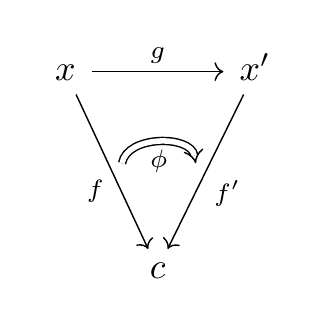
\begin{tikzpicture}
            \node[scale=1.3] (a) at (0,0){
                \begin{tikzcd}[column sep=small]
                    x
                    \ar[ddr, "f"',""{name=f,right}]
                    \ar[rr,"g"]
                    & &
                    x'
                    \ar[ddl,"f'",""{name=fp,left}] \\
                    & \ar[Rightarrow,bend left=80,from=f, to=fp, "\phi"']& \\
                    &  c &
                \end{tikzcd}
            };
        \end{tikzpicture}
        \caption{Lax slice category morphisms in $\mathcal{C}\nnearrow c$}
        \label{fig:lax-slice-def}
    \end{subfigure}%
    \hfill
    \begin{subfigure}[t]{0.47\textwidth}
        \centering
        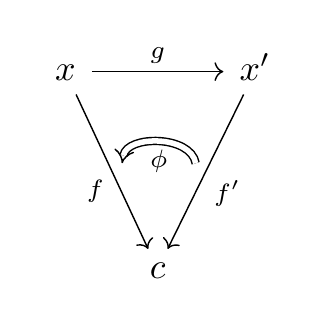
\begin{tikzpicture}
            \node[scale=1.3] (a) at (0,0){
                \begin{tikzcd}[column sep=small]
                    x
                    \ar[ddr, "f"',""{name=f,right}]
                    \ar[rr,"g"]
                    & &
                    x'
                    \ar[ddl,"f'",""{name=fp,left}] \\
                    & \ar[Rightarrow,bend right=80,from=fp, to=f, "\phi"]& \\
                    &  c &
                \end{tikzcd}
            };
        \end{tikzpicture}
        \caption{Op-lax slice category morphisms in %
            $\mathcal{C}\sswarrow c$}
        \label{fig:oplax-slice-def}
    \end{subfigure}
    \begin{subfigure}[t]{0.47\textwidth}
        \centering
        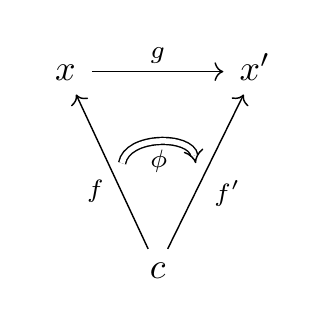
\begin{tikzpicture}
            \node[scale=1.3] (a) at (0,0){
                \begin{tikzcd}[column sep=small]
                    x
                    \ar[from=ddr, "f",""{name=f,right}]
                    \ar[rr,"g"]
                    & &
                    x'
                    \ar[from=ddl,"f'"',""{name=fp,left}] \\
                    & \ar[Rightarrow,bend left=80,from=f, to=fp, "\phi"']& \\
                    &  c &
                \end{tikzcd}
            };
        \end{tikzpicture}
        \caption{Lax coslice category morphisms in $c\nnearrow\mathcal{C}$}
        \label{fig:lax-coslice-def}
    \end{subfigure}%
    \hfill
    \begin{subfigure}[t]{0.47\textwidth}
        \centering
        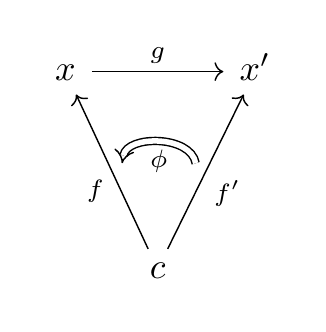
\begin{tikzpicture}
            \node[scale=1.3] (a) at (0,0){
                \begin{tikzcd}[column sep=small]
                    x
                    \ar[from=ddr, "f",""{name=f,right}]
                    \ar[rr,"g"]
                    & &
                    x'
                    \ar[from=ddl,"f'"',""{name=fp,left}] \\
                    & \ar[Rightarrow,bend right=80,from=fp, to=f, "\phi"]& \\
                    &  c &
                \end{tikzcd}
            };
        \end{tikzpicture}
        \caption{Op-lax coslice category morphisms in
            $c \sswarrow \mathcal{C}$}
        \label{fig:oplax-coslice-def}
    \end{subfigure}
    \caption{Lax slice category morphisms definition}
    \label{fig:all-lax-slice-def}
\end{figure*}

Let us try to define PK-nets in this slice paradigm. Let $R$ be an object of $\textbf{CAT}\nnearrow\bf Set$.

The definion \ref{def:lax-slice-2-cat} makes obvious the fact that arrows of the category $\textbf{CAT}\nnearrow\bf Set$ are PK-nets. Consequently, since the objects of any coslice category $R/\big(\textbf{CAT}\nnearrow\bf Set\big)$ are the arrows of $\textbf{CAT}\nnearrow\bf Set$ with their domain in $R$, the objects of  $R/\big(\textbf{CAT}\nnearrow\bf Set\big)$ are PK-nets of form $R$. Let us study the cases of (op-)lax coslice 2-categories on $R$.

\begin{tzcategory}{\caption{PK-nets in the slice categories paradigm}
        \label{fig:slice-PKN}}
    \node[scale=1.3] (a) at (0,0){
        % https://tikzcd.yichuanshen.de/#N4Igdg9gJgpgziAXAbVABwnAlgFyxMJZARgBpiBdUkANwEMAbAVxiRAB12BbOnACwDGjYAGEAviDGl0mXPkIoAzOSq1GLNpx78hDYABEJUmdjwEiZRavrNWiDuwBGAMwAEAZRg5J0kBlPyRAAMpEHW6nYO2oLChgDkkqowUADm8ESgzgBOEFxIISA4EEgATNQ2GvYASiDUDHSOMAwACrJmCiBZWCl83sYg2blIZIXFiGVqtmzutSD1jS1tgfZdPX2+g3mIBUXD5RFsAGKz802tAeYr3b0+mTlbO2PKk5Ughwn9m0jPu+P7U-Z3Ak6g0zktLp1rt5qI0wFB8nUsGBInAIAwsPDPvc9qNvv9XgA5E6gxYXDqrG5iChiIA
        \begin{tikzcd}[row sep = 3em,column sep = 3em]
            \mathcal{D}' \arrow[rddd, "S'"',bend right=6,""{name=Sp}] & & & \\
            & \mathcal{C}
            \arrow[rr, "F"',""{name=F}]
            \arrow[lu, "F'",""{name=Fp,right,near start}]
            &  & \mathcal{D} \arrow[lldd, "S",""{name=S,left}]
            \arrow[lllu, "N"',""{name=N,near start}] \\
            & \arrow[Rightarrow,from=S,to=Sp,"\nu"' near start]
            & \arrow[Rightarrow,to=Fp,from=N,"\mu" near start]
            &  \\
            & \bf Set
            \arrow[from=uu, "R" near end,""{name=R},""{name=R2,left}, crossing over]
            \arrow[Rightarrow,from=R,to=S,"\phi"',crossing over]
            \arrow[Rightarrow,from=R2,to=Sp,"\phi'" near start]
            &  &
        \end{tikzcd}
    };
\end{tzcategory}


\begin{description}
    \item[lax case] : A morphism from $\big<R,S,F,\phi\big>$ to  $\big<R,S',F',\phi'\big>$ in $R\sswarrow(\bf CAT\nnearrow Set)$ is a pair $\big<M,\mu\big>$ where
          $M$ is a PK-net $\big<S,S',N,\nu\big>$  or, in other words, a PK-net $\big<S,S',N,\nu\big>$ (see Figure \ref{fig:slice-PKN}) and
          $\mu : \big<NF,(\nu F)\phi\big> \Rightarrow \big<F',\phi'\big>$ is a 2-morphism of  $\textbf{CAT}\nnearrow\bf Set$ which then must be a natural transformation between $F'$ and $NF$ and must satisfy
          \begin{equation}
              \label{eq:lax-cond}
              \phi' = \big(S'\mu\big)\big((\nu F)\phi\big)
          \end{equation}
    \item[op-lax case] : A morphism from $\big<R,S,F,\phi\big>$ to  $\big<R,S',F',\phi'\big>$ in $R\sswarrow(\bf CAT\nnearrow Set)$ is a pair $\big<M,\mu\big>$ where
          $M$ is an arrow  of $\textbf{CAT}\nnearrow\bf Set$, and
          $\mu : \big<F',\phi'\big>\Rightarrow \big<NF,(\nu F)\phi\big>$ is a natural transformation between $F'$ and $NF$ that satisfies
          \begin{equation}
              \label{eq:oplax-cond}
              (\nu F)\phi = (S'\mu)\phi'
          \end{equation}
\end{description}

In both cases, this gives rise to two notions of PK-homography and also allow to have 2-categories over PK-nets. Moreover, when we consider that $\mu$ is the identity we get from both equations (\ref{eq:lax-cond}) and (\ref{eq:oplax-cond}) the condition of a $\text{PKN}_R$ morphism :
$$\phi' = (\nu F)\phi$$

In fact, we just proved that
\begin{thm}
    $$\text{PKN}_R = R /^s (\bf CAT\nnearrow Set)$$
\end{thm}




\chapter{Extended Klumpenhouwer Networks}
The definition of a PK-net is very general and covers a lot of the concepts introduced, such as (TODO) transposition class, Lewin's GIS (TODO), Forte's (TODO) normal order class, , (TODO) K-nets, symmetric groups of permutations (TODO), Tonnetz...



Let's study a particular class of PK-nets such that $\Delta$, $\mathcal{C}$, $R$ and $S$ are fixed. The only thing we are allowed to change is $F$.

\begin{prop}
    Let $F' : \Delta \rightarrow \mathcal{C}$ such that there exists a natural transformation $\psi : F \rightarrow F'$, then we get an obvious natural transformation $\phi' : R \rightarrow SF$
\end{prop}
% \begin{proof}
%     Let $\phi'_A : R(A) \rightarrow SF'(A)$ such that, $\phi'_A = S\psi_A$. In other words, in the category of functors, $\phi' = Id_S\psi$ which is necessarily a natural transformation, due to the axioms of the category of functors.

% \end{proof}

\begin{tzcategory}{}
    \node[scale=1.3] (a) at (0,0){
        \begin{tikzcd}[column sep = small, row sep = 5.5ex]
            \Delta
            \arrow[bend left=40]{rr}[name=F,label=above:$F$]{}
            \arrow[bend right=40]{rr}[name=F2,label=below:$F'$]{}
            \ar[ddr, "R"',""{name=R,right}]
            & &
            \mathcal{C}
            \arrow[shorten <=5pt,shorten >=0pt,Rightarrow,to path={(F) -- node[label=right:$\psi$] {} (F2)}]{}
            \ar[ddl,"S",""{name=S,left}] \\
            & & \\
            & \textbf{Set}&
        \end{tikzcd}
    };
\end{tzcategory}



\section{Formal definition}

% \begin{defn}[Lawvere theory]
%     A \textbf{Lawvere theory}\cite{hyland2007category} $\mathcal{T}$ is a category with finite products with a distinguished object $x$ such that all objects in $T$ are isomorphic to a finite product $x^n = x \times ... \times x$.
% \end{defn}

\begin{defn}[EK-nets]
    Let $\mathcal{C}$ be a small Lawvere theory. Then, $\bf \text{EKN}_\mathcal{C}$ \label{nomencl:EKN} is defined as the full subcategory of $\textbf{CAT}\nearrow \mathcal{C}$ (see Definition \ref{def:lax-slice-2-cat}) where for all $F\in \text{EKN}_\mathcal{C}$, $F$ is faithful. An object (i.e. a functor $F : \Delta \rightarrow \mathcal{C}$) of the category of the category $\text{EKN}_\mathcal{C}$ is called a $\mathcal{C}$ \textbf{EK-net} on  $\Delta$.
\end{defn}

\begin{rem}
    Note that the functor component $N$ of an arrow between two EK-nets does not have to be faithful.
\end{rem}

For a category $\mathcal{D}$, there may not exist any $\mathcal{C}$ EK-Net on  $\mathcal{D}$.
\begin{defn}[EK candidate]
    A category $\Delta$ is an $\text{EKN}_{\mathcal{C}}$ \textbf{candidate} if there exists at least one $\mathcal{C}$ EK-net on $\Delta$.
\end{defn}

\begin{note}
    From now on, we will presuppose that all the categories named $\Delta$ are candidates for the EK-net category considered.
\end{note}

Intuitively, $\mathcal{C}$ will be the analysis tool we will keep throughout the whole analysis. For a particular EK-net $F : \Delta \rightarrow \mathcal{C}$, $\Delta$ is a pattern matched by the musical object being analysed and $F$ is the musical object analysed itself.




% \begin{defn}[Model of a Lawvere theory]
%     A \textbf{model} of a Lawvere theory $\mathcal{T}$ is a product preserving functor $S : \mathcal{T} \rightarrow \bf Set$.
% \end{defn}

% A particularity of models is that we get a distinguished set $m$  which is the image of the distinguished element $x$. This set can be interpreted as the set of objects the EK-net analyse.

% \begin{defn}[EK-model]
%     Let $F : \Delta \rightarrow \mathcal{C}$ an EK-net. Then an EK-model of $F$ on the model $S$ is the pair $\big<R,\phi\big>$ such that $R$ is full and  the diagram \ref{fig:EK-model-definition} commutes.

%     \begin{tzcategory}{\caption{EK-model definition}
%         \label{fig:EK-model-definition}}
%          \node[scale=1.3] (a) at (0,0){
%         \begin{tikzcd}[column sep=tiny]
%             \Delta
%             \ar[ddr, "R"',""{name=R,right}]
%             \ar[rr,"F"]
%             & &
%             \mathcal{C}
%             \ar[ddl,"S",""{name=S,left}] \\
%             & \ar[Rightarrow,bend left=80,from=R, to=S, "\phi"']& \\
%             & \bf Set &
%         \end{tikzcd}
%          };
%     \end{tzcategory}
% \end{defn}

% In other words, an EK-model is a particular case of PK-net with two main differences : 
% \begin{itemize}
%     \item $\mathcal{C}$ is a Lawvere theory and $S$ is a model of it.
%     \item $R$ is full.
%     \item $F$ is faithfull. 
% \end{itemize}

% In fact, we just get the \textit{object} PK-net but we did not get at all the whole structure (which is the most important part) of PK-homographies and of the $\text{PKN}_{*}$ categories. However, we are not interested in recovering all of this structure. The whole point of the study is to restraint the persepective to get something more usable in practice.

% We are especially insterested here in the set of EK-model that a certain EK-net can generate. The problem is that we have rapidly too many options for $R$ as a candidate

% \begin{exmp}
%     Let $\Delta$ be the category with one element and its identity arrow (we  will call it $*$\label{nomencl:star}). Let $\mathcal{C} = \mathbb{Z}_2$. A model of $\mathbb{Z}_2$ can send the object of $\mathcal{C}$ to any set with more than $2$ elements. Let us pick the case of the standard group action $R_2$ of $\mathbb{Z}_2$ on the set $[\![0,1]\!]$. There is exactly one obvious EK-net between those two categories.

%     There as many functor as singletons betwee $*$  and $\bf Set$.
%     These are our candidate to be EK-models. We still need a natural transformation for each of them. Each time, there is exactly one and is it obvious : the identity.

%     As a conclusion, the class (it is not even a set) of EK-model of this functor has no structure and is hudge.
% \end{exmp}


\section{Constraints on EK-nets}



The purpose of what will follows impose constraints on EK-nets so that we get interesting results musically.

Let $F : \Delta \rightarrow \mathcal{C}$ be an EK-net. Then we call $\Delta$ the (categorical) \textbf{pattern} of $F$ and $\mathcal{C}$ the \textbf{analysis category} of $F$.

\begin{defn}[Relational constraint]
    In $\text{EKN}_\mathcal{C}$, a \textbf{constraint} $\psi$ on a pattern $\Delta$ is a pair of family 
    $$\big<(\sigma_c)_{c\in\mathcal{C}},(\rho_f)_{f\in\bigcup_{(c,c')}Hom(c,c')}\big>$$
    of mappings $\sigma_c$ from $Obj(\Delta)$
    to union of powersets
    $$\bigcup_{c'\in\mathcal{C}}\wp\big(Hom(c,c')\big)$$.
\end{defn}


\begin{defn}[Relational constraint solving]
    Let $\psi$ be a relational constraint of $\text{EKN}_\mathcal{C}$ on a pattern $\Delta$.
    Let us consider the subfamily $\psi_F = (\psi_{F(\delta)})_{\delta\in\Delta}$. Then, $solve(\psi,F)$ is the subcategory of 
    $\text{EKN}_\mathcal{C}$ where
    the objects of $solve(\psi,F)$ are the EK-nets $F' \in \text{EKN}_\mathcal{C}$ such that there exists an arrow $\big< N, \nu\big> : F \rightarrow F'$ such that
    $$\forall \delta \in \Delta, \nu_\delta \in \psi_F(\delta)$$
    which are exactly the arrows of $solve(\psi,F)$.
\end{defn}

Consequenyly, each constraint $\psi_\mathcal{C}$ on $\Delta$ induces a relation
$\_\mathcal{R}_\psi \_$ where $F\mathcal{R}_\psi F'$ if and only if $F'$ is an object of $solve(\psi,F)$.


\begin{defn}[Relational subconstraint]
    Given a constraint $\psi$ in $\text{EKN}_\mathcal{C}$ on a pattern $\Delta$, a constraint $\psi'$ on the same pattern is a \textbf{subconstraint} of $\psi$ if and only if for all $c\in \mathcal{C}$ and $\delta\in\Delta$,
    $$\psi'_c(\delta)\subset\psi_c(\delta)$$
\end{defn}

\begin{prop}
    If $\psi'$ is a relational subconstraint of $\psi$ , then for all EK-net $F$ on the same pattern as $\psi$ and $\psi'$, 
    $$solve(\psi',F)\subset solve(\psi,F)$$
\end{prop}

\paragraph{Constraints representation}

A constraint on $\Delta$ can be represented as the category $\Delta$








\section{How to encode musical objects in the EK-net paradigm}

From now on, we will consider musical object as EK-nets. The fact is that it is not obvious to see how a chord or a picth class is an EK-net. An important part of our work here is to have the possibility to analyse the relations between this objects.

One of the most simple musical object is a pitch class. In a well-tempered tuning, this can be considered as the group $\mathbb{Z}_n$ where $n$ is the number of pitch classes. We have seen that K-nets were a great paradigm to analyse well-tempered music by using the dihedral group and the work of  A. Popoff et al.\cite{PAAE2016} has made a great step toward using this group in music analysis.

Consequently, we will study T/I EK-nets mainly in this report. The first question would then be : are there constraints on T/I EK-nets such that their  solution is exactly 12 (or $n$ in a momre general case).

\subsection{EK pitch classes}

To answer this question, let us first consider the shape the category $\Delta$ that we will be using.

It can be empty, and the only arrow from $\Delta$ to $T/I$ could be interpreted as a timeless silence.

%TODO : better proof
\paragraph{$\Delta$ has only one arrow}
Let us suppose that $\Delta$ as the category with ewacylty one element $\bullet$ and its identity arrow. Consequently, $\Delta$ is isomorphic to a subgroup of $T/I$. The set of the subgroups of $T/I$ is in one-to-one correspondance with the set of $T/I$ EK-Nets with $\Delta$ fixed.
There is only one functor $F:\Delta \rightarrow T/I$ which maps $Id_\bullet$ to $T_0$.

In other words, there exactly one EK-net of this $\Delta$. If we need a musical to be completely unique, we can encode it as a unique object with a unique arrow. It could be interpreted as a silence.


%For instance, if track is using a certain key (e.g. Amin), we could map this key to this object so it acts as an anchor.

\paragraph{$\Delta$ has two arrows}
There are $13$ 2-elements subgroups of $T/I$ : $\{T_0,T_6\}$ and $\forall k\in[\![1,12]\!], \{T_0,I_k\}$. They are all obviously isomorphic to the group $\mathbb{Z}_2$, that we can safely choose as our $\Delta$. Consequently, we get $13$ parallel functors from $\mathbb{Z}_2$ to $T/I$.

We also know that all (inner) automorphisms of T/I are natural transformations between endofunctors of $T/I$. Precisely, all the functors corresponding to the subgroups $\{T_0,I_k\}$ are isomorphic threw a positive automorphism.
%TODO define positive isomorphisms

However, since all automorphisms of T/I send transpositions on transpositions and inversions on inversions, there is no natural transformations for $\{T_0,T_6\}$ to any other functor.
%TODO maybe name better those functors

Consequently, we have two equivalence classes of EK-nets. This gives to the analyst two different tools to analyse a point with two arrows on it.

It would be tempting to define our pitch-classes as the 12 functors with a maping like this :

%TODO define f and everything

\begin{eqnarray*}
    C & \rightarrow (f \rightarrow I_0) \\
    C\sharp &\rightarrow (f \rightarrow I_1) \\
    &\vdots \\
    B & \rightarrow (f \rightarrow I_{11})
\end{eqnarray*}

\begin{tzcategory}{\caption{Constraint with two arrows}
        \label{fig:2-arrow-constr}}
    \node[scale=1.3] (a) at (0,0){
        % https://tikzcd.yichuanshen.de/#N4Igdg9gJgpgziAXAbVABwnAlgFyxMJZABgBpiBdUkANwEMAbAVxiRAB12AjJhhmHCAC+VEDCgBzeEVAAzAE4QAtkjIgcEVdQYQIaIgEYAHGVmM4MUQzpcYDAAqZc+QohDysEgBaCRQoA
        \begin{tikzcd}
            \bullet \arrow["I\_"',loop, distance=2em, in=125, out=55]
        \end{tikzcd}
    };
\end{tzcategory}

Indeed, the constraint in Figure \ref{fig:2-arrow-constr} has 12 solutions, as we have seen above. So each of these EK-nets are a candidate to be a pitch-class.


However, this would not be coherent with the interaction between two pitch-classes. Indeed, if we want to use two different pitch-classes, with an arrow between them, we are forced by the category constraints to have at least two morphisms between the pitch-classes, as we can see in Figure \ref{wrongPitchClass}.
%TODO : finish paragraph

\begin{tzcategory}{\caption{Wrong definition of pitch classes}
        \label{wrongPitchClass}}
    \node[scale=1.3] (a) at (0,0){
        \begin{tikzcd}
            {}
            \bullet \arrow["I_i"', loop, distance=2em, in=125, out=55] &      \\
            &      \\
            \bullet \arrow["I_j"', loop, distance=2em, in=305, out=235] \arrow[uu, "I_y"', bend right] \arrow[uu, "T_x", bend left] &
        \end{tikzcd}
    };
\end{tzcategory}


\begin{prop}
    By considering a pitch class as a single point with to reflexive arrows, we can use only half of the notes in practice.
\end{prop}
\begin{proof}
    $i$ and $j$ are fixed.
    \begin{eqnarray*}
        I_i \circ T_x  = I_y \Rightarrow i - x = y \Rightarrow i = x + y\\
        T_x \circ I_j = I_y \Rightarrow x + j = y \Rightarrow j = y - x\\
    \end{eqnarray*}
    So we get
    $$\systeme*{2x = i - j, 2y = i + j}$$

    This is possible iff $i$ and $j$ have the same parity. In other words, in a connex component of the category $\Delta$, we could only use 6 notes.


\end{proof}

This can be explained by the fact that here the theory considers the interval by going from one note to the other by the fastest path, which we are not used to do. It could be fun by the way to transform a sing in another by this consideration.

A fix to this problem is to consider a pitch class constraint as a 2-objects EK-net (see Figure \ref{fig:constrPitchClass}).

\begin{tzcategory}{\caption{Constraint for EK relative pitch classes}
        \label{fig:constrPitchClass}}
    \node[scale=1.3] (a) at (0,0){
        % https://tikzcd.yichuanshen.de/#N4Igdg9gJgpgziAXAbVABwnAlgFyxMJZABgBoA2AXVJADcBDAGwFcYkQAdDgI2ccZg4QAX1LpMufIRRkALNTpNW7Lr36CRYkBmx4CRAIyliChizaIQm8bqlEyJmmeWWRCmFADm8IqABmAE4QALZIZCA4EGE0jBAQaPakfkxwMAqM9NwwjAAKEnrSIAFYngAWQk5KFiAAKgD6wORYwtYggSFIRhFRiF2x8YYAHGTJjKnpmdl5tvqWxWUViubsAJINAEwA1i2i-kGhiOGRnTRZYFBIALQAzOHO1fWNzSAxk7n5dnMl5a3tB0c9LpnC6IW6vLLvGaFAR+Rb3VYbTaXJotGg4ehYRjsSBgNi7Nr7JDrNE9a7CSjCIA
        \begin{tikzcd}
            {}
            \bullet
            \arrow["I\_"',loop, distance=2em, in=125, out=55]  & \\
            &  \\
            \bullet
            \arrow[uu, bend right] \arrow[uu, bend left] &
        \end{tikzcd}
    };

\end{tzcategory}

\begin{prop}
    The solutions for the constraint in Figure \ref{fig:constrPitchClass} are the EK-nets of the form described in Figure \ref{fig:solConstrPitch}.
    \begin{tzcategory}{\caption{Constraint solution for EK relative pitch classes}
            \label{fig:solConstrPitch}}
        \node[scale=1.3] (a) at (0,0){
            % https://tikzcd.yichuanshen.de/#N4Igdg9gJgpgziAXAbVABwnAlgFyxMJZABgBoA2AXVJADcBDAGwFcYkQAdDgI2ccZg4QAX1LpMufIRRkALNTpNW7Lr36CRYkBmx4CRAIyliChizaIQm8bqlEyJmmeWWRCmFADm8IqABmAE4QALZIZCA4EGE0jBAQaPakfkxwMAqM9NwwjAAKEnrSIAFYngAWQk5KFiAAKgD6wORYwtYggSFIRhFRiF2x8YYAHGTJjKnpmdl5tvqWxWUViubsAJINAEwA1i2i-kGhiOGRnTRZYFBIALQAzOHO1fWNzSAxk7n5dnMl5a3tB0c9LpnC6IW6vLLvGaFAR+Rb3VYbTaXJotGg4ehYRjsSBgNi7Nr7JDrNE9a7CSjCIA
            \begin{tikzcd}
                \bullet
                \arrow["I_i"',loop, distance=2em, in=125, out=55]  & &\\
                &    &  x + y = i\\
                \bullet
                \arrow[uu, "I_y"', bend right] \arrow[uu, "T_x", bend left] &&
            \end{tikzcd}
        };

    \end{tzcategory}
\end{prop}

\begin{proof}
    Since there are two different arrows between the objects, there must be one transposition and one inversion because the EK-net is faithful. This demonstrates the form of the solution in figure \ref{fig:solConstrPitch}.The functor requirements forces the following system to be satisfied : 
    $$\systeme*{i-x = y,i-y = x }$$
    which has the obvious solution $i = x + y$

\end{proof}

Elementary algebra tells us that for every $i$ possible, there are $12$ choices for $x$ and $y$. In other words, this constraint yields a $144 = 12^2$ elements solution set. We could interpret this set as a pair of every possible pitch-classes. Instead, we will call the object with only one arrow the root note and the one with two arrows as the pitch relative to the root note.

\begin{defn}[Relative pitch-class]
    A \textbf{relative pitch-class} is one of the solutions of the relative pitch-class constraint (see Figure \ref{fig:constrPitchClass}).
\end{defn}

We now have $12$ candidates for each pitch class, because for one relative pitch-class, we must fix a root note. The idea behind this construction is that we just need to transpose the root note to get the transposition of the whole EK-nets.

Indeed, we did not yet use the whole power of EK-constraints

% https://tikzcd.yichuanshen.de/#N4Igdg9gJgpgziAXAbVABwnAlgFyxMJZABgBoAmAXVJADcBDAGwFcYkQAVAfQGsQBfUuky58hFGWLU6TVu27EB0mFADm8IqABmAJwgBbJGRA4ISAIw0ARjDBQkAZmMMWbRJy4APAUJC6DRjSmFta29ogAtE40LnLu3ACeIDSM9DaMAAoieATsOliqABY4Ptp6hoiWJmaVKRAQaETmABxkWkxwMNKp6VnYOeIg+UUlMbJuIACSXPRK-EA
\begin{tikzcd}
    T_0 \arrow["I_a"', loop, distance=2em, in=125, out=55]          \\
                                                                    \\
    T_k \arrow[uu, "T_x", bend left] \arrow[uu, "T_y"', bend right]
    \end{tikzcd}


% \begin{tzcategory}{\caption{The k pitch-classes as PK-nets}
%         \label{pitchClassDef}}
%     \node[scale=1.3] (a) at (0,0){
%         % https://tikzcd.yichuanshen.de/#N4Igdg9gJgpgziAXAbVABwnAlgFyxMJZABgBoA2AXVJADcBDAGwFcYkQAdDgI2ccZg4QAX1LpMufIRRkALNTpNW7Lr36CRYkBmx4CRAIyliChizaIQm8bqlEyJmmeWWRCmFADm8IqABmAE4QALZIZCA4EGE0jBAQaPakfkxwMAqM9NwwjAAKEnrSIAFYngAWQk5KFiAAKgD6wORYwtYggSFIRhFRiF2x8YYAHGTJjKnpmdl5tvqWxWUViubsAJINAEwA1i2i-kGhiOGRnTRZYFBIALQAzOHO1fWNzSAxk7n5dnMl5a3tB0c9LpnC6IW6vLLvGaFAR+Rb3VYbTaXJotGg4ehYRjsSBgNi7Nr7JDrNE9a7CSjCIA
%         \begin{tikzcd}
%             {}
%             X \arrow["I_{2i}"', loop, distance=2em, in=125, out=55] &      \\
%             &      \\
%             Y %\arrow["T_{k}"', loop, distance=2em, in=305, out=235] 
%             \arrow[uu, "I_{i}"', bend right] \arrow[uu, "T_{i}", bend left] &
%         \end{tikzcd}
%     };

% \end{tzcategory}

\begin{prop}
    By fixing $\Delta$ as shown in Figure% \ref{pitchClassDef}, we get an analysis set of 12 EK-Nets.
\end{prop}

\begin{proof}
    A transposition of $j$ semi-tones of a pitch class $i$ is a natural transformation $$\psi = \systeme*{X\rightarrow T_j, Y\rightarrow T_0}$$

    \begin{tzcategory}{\caption{The k pitch-classes as PK-nets}
        }
        \node[scale=1.3] (a) at (0,0){
            % https://tikzcd.yichuanshen.de/#N4Igdg9gJgpgziAXAbVABwnAlgFyxMJZABgBpiBdUkANwEMAbAVxiRADEAKADQEoQAvqXSZc+QigBM5KrUYs27AOQ9+QkdjwEiZSbPrNWiDpwCaa4SAybxRaXuoGFx5WYsax2lGQDM++UYmfIKW1p4SyNJ+jgGKKsHqVqJaEWQArP6Gim4hHil2pBkxWS4q5oKyMFAA5vBEoABmAE4QALZIZCA4EEjSciUgAJIA+sCSWAIg1Ax0AEYwDAAKybbGTVjVABY4uSDNbR3U3UgAjMXOIAAqwwBWUyAz80srXg8wDTuJ++2IZ109iB850CIzGnCwAGobrxJtM5gtljZXgx3p9LN9ekcAUD+hdrnc4U9EeE2OstmjGi0fgAWLFIABswLY1yw90eCJeEhAZO2uwxiFp-yQaSZxmuxDZ8OeSK5KI+fKpwrpiAA7KKrqNITdYQ8pcT8sY5RS9orEIyhar1fjJUTOaSNryBBQBEA
            \begin{tikzcd}
                F(X) \arrow[dd, "I_{2i}"'] \arrow[rr, "T_j"]
                &  & F'(X) \arrow[dd, "I_{2(i+j)}"]
                &  & F(X) \arrow[dd, "T_i"'] \arrow[rr, "T_0"]
                &  & F'(X) \arrow[dd, "T_{i+j}"]   \\
                \\
                F(Y) \arrow[rr, "T_j"']
                &  & F'(Y)
                &  & F(Y) \arrow[rr, "T_j"']
                &  & F'(Y)
            \end{tikzcd}
        };
    \end{tzcategory}
\end{proof}








\subsection{EK-nets on monoids}
In EK-nets, we are particularly interested in the case where $\mathcal{C} = T/I$. Since $T/I$ has only one element, all the functors $F:\Delta \rightarrow T/I$ send all the elements on the unique element of $T/I$. In the following, we will not recall the image of the elements of $\Delta$.

EK-nets have particular properties when the category $\mathcal{C}$ has a single element. Let $\mathcal{M}$ be such a category and let us consider  an $\mathcal{M}$ EK-nets .

If $\Delta$ has a single element, then the functors $[\Delta,\mathcal{M}]$ are in one-to-one correspondance with the monoid morphisms. Since EK-nets are faithful, we only get the injective morphisms. In other words, the set of $\text{EKN}_{\mathcal{M}}$ candidates is in one-to-one correspondence with the submonoids of $M$.

\begin{prop}
    The natural transformation components $\nu : F \rightarrow F'N$ of EK-homographies do not actually depend on $F$ when we consider $\mathcal{M}$ EK-nets.
\end{prop}

Indeed, since $\mathcal{M}$ has only one element $\bullet$, any mapping from $\Delta$'s elements to a reflexive arrows of $\bullet$ defines a set of endomorphisms from any $T/I$ EK-net on $\Delta$.
%TODO define group action
% Here, $S:\mathcal{C}\rightarrow \textbf{Set}$ is the action of $T/I$ on the set $Notes = \{C,C\sharp,D,E\flat,E,F,F\sharp,G\sharp,A,B\flat,B\}$.

\subsection{EK-nets on groups}

Let $F:\Delta\rightarrow G$ and $F':\Delta\rightarrow G$ be two parallel functors where $G\in \textbf{Grp}$. Let $X,Y\in\Delta$ and $f\in Hom(X,Y)$. We then get the following commutating diagram :

\begin{tzcategory}{}
    \node[scale=1.3] (a) at (0,0){
        \begin{tikzcd}[column sep = small]
            F(X) \arrow[dd, "F(f)"'] \arrow[rr, "\psi_X"] &  & F'(X) \arrow[dd, "F'(f)"] \\
            &  &                           \\
            F(Y) \arrow[rr, "\psi_Y"']                    &  & F'(Y)
        \end{tikzcd}
    };
\end{tzcategory}


This diagram corresponds to the equation :
\begin{eqnarray*}
    &\psi_Y\cdot F(f) &=   F'(f) \cdot \psi_X \\
    \Leftrightarrow &
    F'(f) &=   \psi_Y\cdot F(f) \cdot \psi_X^{-1}\\
\end{eqnarray*}

Hence, there is no constraint on the couple $(x,y)$, we juste need to choose $a = x$ and $b = y$, and we get our natural transformation.

Though, $X$ and $Y$ are actually the same object and $f$ is a reflexive object, we get $a = b$, and consequently,
$$y = b^{-1}\cdot x \cdot b $$

In other words, $\psi$ is an \textbf{inner automorphism} of $G$.


\subsection{Transposition generalization}

\begin{defn}[EK pitch class]

\end{defn}

\begin{defn}[EK-anchor]
    An \textbf{EK-anchor} is an object $a\in\Delta$  with only one reflexive arrow on $a$ in $\Delta$ (a.k.a $id_a$).
\end{defn}

Fundamentally, an anchor is a musical object that can be interpreted freely.

\begin{prop}[EK-anchor properties]~
    \begin{enumerate}
        % \item Let $a$ be an EK-anchor. For any object $d \in \Delta$, there is at most one arrow $f:d\rightarrow a$.
        \item For any $a\in \Delta$, if there exists an object $d\in \Delta$ such that $\textbf{card}([d,a]) = 1$, then $a$ is an EK-anchor.
    \end{enumerate}
    \label{anchorProp}
\end{prop}

\begin{proof}
    \begin{enumerate}
        %\item The unicity is immediate from the composition law of a category.
        \item By absurd, if we suppose $a$ is not an anchor, then it has at least one reflexive arrow $r$ different from the identity. Let $f : d\rightarrow a$ the unique arrow between $d$ and $a$. Then we must have $r \circ f = f$ since $f$ is unique. So $r$ would have to be the identity.
    \end{enumerate}
\end{proof}

\begin{defn}[Generalization of transposition]
    For any T/I EK-net $F$ on $\Delta$, a transposition $\tau$ is a mapping from $Obj(\Delta)$ to $ $
\end{defn}


\section{Constraints}

\begin{defn}[EK-domain]
    An $EKN_\mathcal{C}$ musical domain
\end{defn}

\begin{defn}

\end{defn}


\section{Recovering intervals}

Let us study how to use PK-nets with a 2-objects category $\Delta$.




% TODO  : what is the juxtaposition of two connected component (ie no morphism between them)


\section{Recover Tonnetz}


\begin{defn} The \textbf{category of elements} $el(F)$ of a functor $F : \mathcal{C}\rightarrow \textbf{Set}$ is defined as follows :
    \begin{itemize}
        \item its objects are the pairs $(c,x)$ where $c$ is an object of $\mathcal{C}$ and $x\in F(c)$
        \item its morphisms $(c,x)\rightarrow (c',x')$ are morphisms $u : c\rightarrow c'$ such that $F(u)(x) = x'$
    \end{itemize}
\end{defn}
\paragraph{}
Now, what is the category of elements of the PLR-group action over \textbf{Set}? Let $S$ be the functor from the category PLR to the category \textbf{Set} such that $S$ associates to the only object of PLR a set $X$ of cardinality 24 and such that $S$ is a PLR-group action on $X$.

$el(S)$ is then a category with $24$ objects. One can use it as a $\Delta$ category in a PK-net. The transformation $\phi$ gives us the musical interpretation, of each transformation triads.

=> How to add more structure to eliminate arrow? Maybe take two generators

\chapter{EK-nets as musical objects}


From now on, we will consider musical object as EK-nets. The fact is that it is not obvious to see how a chord or a picth class is an EK-net. An important part of our work here is to have the possibility to analyse the relations between this objects.

One of the most simple musical object is a pitch class. In a well-tempered tuning, this can be considered as the group $\mathbb{Z}_n$ where $n$ is the number of pitch classes. We have seen that K-nets were a great paradigm to analyse well-tempered music by using the dihedral group and the work of  A. Popoff et al.\cite{PAAE2016} has made a great step toward using this group in music analysis.

Consequently, according to  we will study T/I EK-nets mainly in this section.

The first question that we want to tackle : are there (structural or relational) constraints on T/I EK-nets such that their solution is exactly 12 (or $n$ in a more general case).

\section{EK pitch classes}

To answer this question, let us first consider the shape the category $\Delta$ that we should be using. It can be empty, and the only arrow from $\Delta$ to $T/I$ could be interpreted as a timeless silence.

%TODO : better proof
\paragraph{$\Delta$ has one object and one arrow}
Let us suppose that $\Delta$ as the category with exactly one element $\bullet$ and its identity arrow. Consequently, $\Delta$ is isomorphic to a subgroup of $T/I$. The set of the subgroups of $T/I$ is in one-to-one correspondance with the set of $T/I$ EK-Nets with $\Delta$ fixed.
There is only one functor $F:\Delta \rightarrow T/I$ which maps $Id_\bullet$ to $T_0$.

In other words, there exactly one EK-net of this $\Delta$. If we need a musical to be completely unique, we can encode it as a unique object with a unique arrow. It could be interpreted as an anchor to build upon, a little bit like an anchor or a landmark that has only one interpretation.


%For instance, if track is using a certain key (e.g. Amin), we could map this key to this object so it acts as an anchor.

\paragraph{$\Delta$ has one object two arrows}
There are $13$ 2-elements subgroups of $T/I$ : $\{T_0,T_6\}$ and $\forall k\in[\![1,12]\!], \{T_0,I_k\}$. They are all obviously isomorphic to the group $\mathbb{Z}_2$, that we can safely choose as our $\Delta$. Consequently, according to Proposition \ref{prop:submon} we get $13$ parallel functors from $\mathbb{Z}_2$ to $T/I$.

We also know that all inner automorphisms of T/I are natural transformations between endofunctors of $T/I$ \ref{prop:inner-auto}. Precisely, all the functors corresponding to the subgroups $\{T_0,I_k\}$ are isomorphic threw a positive automorphism.
%TODO define positive isomorphisms

However, since all automorphisms of T/I send transpositions on transpositions and inversions on inversions, there is no natural transformations for $\{T_0,T_6\}$ to any other functor.
%TODO maybe name better those functors

Consequently, we have two equivalence classes of EK-nets. This gives to the analyst two different tools to analyse a point with two arrows on it.

It would be tempting to define our pitch-classes as the 12 functors with a maping like this :

%TODO define f and everything

\begin{eqnarray*}
    C & \rightarrow (f \rightarrow I_0) \\
    C\sharp &\rightarrow (f \rightarrow I_1) \\
    &\vdots \\
    B & \rightarrow (f \rightarrow I_{11})
\end{eqnarray*}

\begin{tzcategory}{\caption{Structural constraint with 12 solutions}
        \label{fig:2-arrow-constr}}
    \node[scale=1.3] (a) at (0,0){
        % https://tikzcd.yichuanshen.de/#N4Igdg9gJgpgziAXAbVABwnAlgFyxMJZABgBpiBdUkANwEMAbAVxiRAB12AjJhhmHCAC+VEDCgBzeEVAAzAE4QAtkjIgcEVdQYQIaIgEYAHGVmM4MUQzpcYDAAqZc+QohDysEgBaCRQoA
        \begin{tikzcd}
            \bullet \arrow["I\_"',loop, distance=2em, in=125, out=55]
        \end{tikzcd}
    };
\end{tzcategory}

Indeed, the constraint in Figure \ref{fig:2-arrow-constr} has 12 solutions, as we have seen above. So each of these EK-nets are a candidate to be a pitch-class.


However, we would also like that there exists some relational constraint to express intervals. Indeed, if we want to use two different pitch-classes, with an arrow between them, we are forced by the category constraints to have at least two morphisms between the pitch-classes, as we can see in Figure \ref{wrongPitchClass}.
%TODO : finish paragraph

\begin{tzcategory}{\caption{Wrong definition of pitch classes}
        \label{wrongPitchClass}}
    \node[scale=1.3] (a) at (0,0){
        \begin{tikzcd}
            {}
            \bullet \arrow["I_i"', loop, distance=2em, in=125, out=55] &      \\
            &      \\
            \bullet \arrow["I_j"', loop, distance=2em, in=305, out=235] \arrow[uu, "I_y"', bend right] \arrow[uu, "T_x", bend left] &
        \end{tikzcd}
    };
\end{tzcategory}


\begin{prop}
    By considering a pitch class as a single point with two reflexive arrows, we can use only half of the notes in practice.
\end{prop}
\begin{proof}
    $i$ and $j$ are fixed.
    \begin{eqnarray*}
        I_i \circ T_x  = I_y \Rightarrow i - x = y \Rightarrow i = x + y\\
        T_x \circ I_j = I_y \Rightarrow x + j = y \Rightarrow j = y - x\\
    \end{eqnarray*}
    So we get
    $$\systeme*{2x = i - j, 2y = i + j}$$

    This is possible iff $i$ and $j$ have the same parity. In other words, in a connex component of the category $\Delta$, we could only use 6 notes, even with the broader constraint we can use.
\end{proof}

This can be explained by the fact that here the theory considers the interval by going from one note to the other without having a direction of rotation, using a kind of absolute value : $11$ becomes $1$, $10$ becomes $2$, etc. This has already been observed by \cite{forte_1980}.

A fix to this problem is to consider a pitch class constraint as a 2-objects EK-net (see Figure \ref{fig:constrPitchClass}).

\begin{tzcategory}{\caption{Structural constraint for EK relative pitch classes}
        \label{fig:constrRelPitchClass}}
    \node[scale=1.3] (a) at (0,0){
        % https://tikzcd.yichuanshen.de/#N4Igdg9gJgpgziAXAbVABwnAlgFyxMJZABgBoA2AXVJADcBDAGwFcYkQAdDgI2ccZg4QAX1LpMufIRRkALNTpNW7Lr36CRYkBmx4CRAIyliChizaIQm8bqlEyJmmeWWRCmFADm8IqABmAE4QALZIZCA4EGE0jBAQaPakfkxwMAqM9NwwjAAKEnrSIAFYngAWQk5KFiAAKgD6wORYwtYggSFIRhFRiF2x8YYAHGTJjKnpmdl5tvqWxWUViubsAJINAEwA1i2i-kGhiOGRnTRZYFBIALQAzOHO1fWNzSAxk7n5dnMl5a3tB0c9LpnC6IW6vLLvGaFAR+Rb3VYbTaXJotGg4ehYRjsSBgNi7Nr7JDrNE9a7CSjCIA
        \begin{tikzcd}
            {}
            \bullet
            \arrow["I\_"',loop, distance=2em, in=125, out=55]  & \\
            &  \\
            \bullet
            \arrow[uu, bend right] \arrow[uu, bend left] &
        \end{tikzcd}
    };

\end{tzcategory}

\begin{prop}
    The solutions for the structural constraint in Figure \ref{fig:constrRelPitchClass} are the EK-nets of the form described in Figure \ref{fig:solConstrRelPitch}.
    \begin{tzcategory}{\caption{Solution to \ref{fig:constrRelPitchClass} (called EK relative pitch classes)}
            \label{fig:solConstrRelPitch}}
        \node[scale=1.3] (a) at (0,0){
            % https://tikzcd.yichuanshen.de/#N4Igdg9gJgpgziAXAbVABwnAlgFyxMJZABgBoA2AXVJADcBDAGwFcYkQAdDgI2ccZg4QAX1LpMufIRRkALNTpNW7Lr36CRYkBmx4CRAIyliChizaIQm8bqlEyJmmeWWRCmFADm8IqABmAE4QALZIZCA4EGE0jBAQaPakfkxwMAqM9NwwjAAKEnrSIAFYngAWQk5KFiAAKgD6wORYwtYggSFIRhFRiF2x8YYAHGTJjKnpmdl5tvqWxWUViubsAJINAEwA1i2i-kGhiOGRnTRZYFBIALQAzOHO1fWNzSAxk7n5dnMl5a3tB0c9LpnC6IW6vLLvGaFAR+Rb3VYbTaXJotGg4ehYRjsSBgNi7Nr7JDrNE9a7CSjCIA
            \begin{tikzcd}
                \bullet
                \arrow["I_{i+2y}"',loop, distance=2em, in=125, out=55]  & &\\
                &    &  \\
                \bullet
                \arrow[uu, "I_{y}"', bend right] \arrow[uu, "T_{i+y}", bend left] &&
            \end{tikzcd}
        };

    \end{tzcategory}
\end{prop}

\begin{proof}
    Since there are two different arrows between the objects, there must be one transposition and one inversion because the EK-net is faithful. This demonstrates the form of the solution in figure \ref{fig:solConstrRelPitch}. By fixing to $T_x$ the left arrow and $I_y$ the right one, the functor requirements forces the following system to be satisfied :
    $$\systeme*{i-x = y,i-y = x }$$
    which has the obvious solution $y = x - i$, which is equivalent to $x = y + i$

\end{proof}

This constraint then yields a $144 = 12^2$ elements solution set. We could interpret this set as the the set of the pairs of every possible pitch-classes. Instead, we will call the object with only one arrow the root note and the one with two arrows as the pitch relative to the root note.

\begin{defn}[Relative pitch-class]
    A \textbf{relative pitch-class} is one of the solutions of the relative pitch-class constraint (see Figure \ref{fig:constrRelPitchClass}) illustrated in
\end{defn}




This illustrates a problem which, in our knowledge has not been tackled : if the pitch classes are a group, how do we choose the neutral element of the group. We could choose C but there is no reason we wouldn't choose another one.
This is similar to a change of referential in mecanics : if we want a car to move, we can either ask someone to drive the car moving and observing it moving or just walk a bit, the car will still be moving in our referential.





We now have $12$ candidates for each pitch class, because for one relative pitch-class, we must fix a root note. The idea behind this construction is that we just need to transpose the root note to get the transposition of the whole EK-nets.

\begin{defn}[Pitch-class]
    The $k^{th}$ \textbf{pitch-class} is the solution of the subconstraint of the constraint in Figure \ref{fig:constrPitchClass} illustrated by Figure \ref{fig:constrPitchClass}

    \begin{tzcategory}{\caption{Structural constraint for the $k^{th}$ pitch classes}
            \label{fig:constrPitchClass}}
        \node[scale=1.3] (a) at (0,0){
            % https://tikzcd.yichuanshen.de/#N4Igdg9gJgpgziAXAbVABwnAlgFyxMJZABgBoA2AXVJADcBDAGwFcYkQAdDgI2ccZg4QAX1LpMufIRRkALNTpNW7Lr36CRYkBmx4CRAIyliChizaIQm8bqlEyJmmeWWRCmFADm8IqABmAE4QALZIZCA4EGE0jBAQaPakfkxwMAqM9NwwjAAKEnrSIAFYngAWQk5KFiAAKgD6wORYwtYggSFIRhFRiF2x8YYAHGTJjKnpmdl5tvqWxWUViubsAJINAEwA1i2i-kGhiOGRnTRZYFBIALQAzOHO1fWNzSAxk7n5dnMl5a3tB0c9LpnC6IW6vLLvGaFAR+Rb3VYbTaXJotGg4ehYRjsSBgNi7Nr7JDrNE9a7CSjCIA
            \begin{tikzcd}
                {}
                \bullet
                \arrow["I\_"',loop, distance=2em, in=125, out=55]  & \\
                &  \\
                \bullet
                \arrow[uu, bend right,"I_k"'] \arrow[uu, bend left] &
            \end{tikzcd}
        };
    \end{tzcategory}
\end{defn}


This allows us to propose a new approach to transposition, instead of saying that transposing a track is transposing each note after the other, we just use relative pitch-class whose anchor $y$ is fixed. To transpose the track we then just have to transpose the anchor and all the relative pitch classes will follow automatically.


%Indeed, we did not yet use the whole power of EK-constraints



\section{Transposition generalization}

\begin{defn}[EK-anchor]
    An \textbf{EK-anchor} is an object $a\in\Delta$  with only one reflexive arrow (which must be $id_a$).
\end{defn}

Fundamentally, an anchor is a landmark on the dodecahedron.

% \begin{prop}[EK-anchor properties]~
%     \begin{enumerate}
%         % \item Let $a$ be an EK-anchor. For any object $d \in \Delta$, there is at most one arrow $f:d\rightarrow a$.
%         \item For any $a\in \Delta$, if there exists an object $d\in \Delta$ such that $\textbf{card}([d,a]) = 1$, then $a$ is an EK-anchor.
%     \end{enumerate}
%     \label{anchorProp}
% \end{prop}

% \begin{proof}
%     \begin{enumerate}
%         %\item The unicity is immediate from the composition law of a category.
%         \item By absurd, if we suppose $a$ is not an anchor, then it has at least one reflexive arrow $r$ different from the identity. Let $f : d\rightarrow a$ the unique arrow between $d$ and $a$. Then we must have $r \circ f = f$ since $f$ is unique. So $r$ would have to be the identity.
%     \end{enumerate}
% \end{proof}

% \begin{proof}
%     A transposition of $j$ semi-tones of a pitch class $i$ is a natural transformation $$\psi = \systeme*{X\rightarrow T_j, Y\rightarrow T_0}$$

%     \begin{tzcategory}{\caption{The k pitch-classes as PK-nets}
%         }
%         \node[scale=1.3] (a) at (0,0){
%             % https://tikzcd.yichuanshen.de/#N4Igdg9gJgpgziAXAbVABwnAlgFyxMJZABgBpiBdUkANwEMAbAVxiRADEAKADQEoQAvqXSZc+QigBM5KrUYs27AOQ9+QkdjwEiZSbPrNWiDpwCaa4SAybxRaXuoGFx5WYsax2lGQDM++UYmfIKW1p4SyNJ+jgGKKsHqVqJaEWQArP6Gim4hHil2pBkxWS4q5oKyMFAA5vBEoABmAE4QALZIZCA4EEjSciUgAJIA+sCSWAIg1Ax0AEYwDAAKybbGTVjVABY4uSDNbR3U3UgAjMXOIAAqwwBWUyAz80srXg8wDTuJ++2IZ109iB850CIzGnCwAGobrxJtM5gtljZXgx3p9LN9ekcAUD+hdrnc4U9EeE2OstmjGi0fgAWLFIABswLY1yw90eCJeEhAZO2uwxiFp-yQaSZxmuxDZ8OeSK5KI+fKpwrpiAA7KKrqNITdYQ8pcT8sY5RS9orEIyhar1fjJUTOaSNryBBQBEA
%             \begin{tikzcd}
%                 F(X) \arrow[dd, "I_{2i}"'] \arrow[rr, "T_j"]
%                 &  & F'(X) \arrow[dd, "I_{2(i+j)}"]
%                 &  & F(X) \arrow[dd, "T_i"'] \arrow[rr, "T_0"]
%                 &  & F'(X) \arrow[dd, "T_{i+j}"]   \\
%                 \\
%                 F(Y) \arrow[rr, "T_j"']
%                 &  & F'(Y)
%                 &  & F(Y) \arrow[rr, "T_j"']
%                 &  & F'(Y)
%             \end{tikzcd}
%         };
%     \end{tzcategory}
% \end{proof}

\begin{defn}[Generalization of transposition]
    Let $\tau^k$ be a relational constraint in $\text{EKN}_\mathcal{C}$ on a pattern $\Delta$ such that, for every $c\in\mathcal{C}$
    \begin{itemize}
        \item for every anchor $a$ in $\Delta$, $\tau^k_c(a) = \{T_{k}\}$
        \item for all the other objects $d$ of $\Delta$, $\tau^k_c(d) = \{T_0\}
              $
    \end{itemize}
    Then $\tau$ is called the transposition constraint.
\end{defn}

\begin{exmp}
    \begin{tzcategory}{\caption{The 12 EK-nets corresponding to F}
            \label{fig:solF}}
        \node[scale=1.3] (a) at (0,0){
            % https://tikzcd.yichuanshen.de/#N4Igdg9gJgpgziAXAbVABwnAlgFyxMJZABgBoA2AXVJADcBDAGwFcYkQAdDgI2ccZg4QAX1LpMufIRRkALNTpNW7Lr36CRYkBmx4CRAIyliChizaIQm8bqlEyJmmeWWRCmFADm8IqABmAE4QALZIZCA4EGE0jBAQaPakfkxwMAqM9NwwjAAKEnrSIAFYngAWQk5KFiAAKgD6wORYwtYggSFIRhFRiF2x8YYAHGTJjKnpmdl5tvqWxWUViubsAJINAEwA1i2i-kGhiOGRnTRZYFBIALQAzOHO1fWNzSAxk7n5dnMl5a3tB0c9LpnC6IW6vLLvGaFAR+Rb3VYbTaXJotGg4ehYRjsSBgNi7Nr7JDrNE9a7CSjCIA
            \begin{tikzcd}
                r\arrow["I_{i+10}"',loop, distance=2em, in=125, out=55]  & &\\
                &    &  \\
                a \arrow[uu, "I_{5}"', bend right]
                \arrow[uu, "T_{i+5}", bend left] &&
            \end{tikzcd}
        };

    \end{tzcategory}
    Let us see how to get the transposition of 8 semitones of the note F. We know that the note $C$ is the solution to the structural constraint of Figure \ref{fig:constrPitchClass}. Therefore, it is the set of all EK-nets with $i\in[\![0,11]\!]$ presented in Figure \ref{fig:solF}.

    We know that $\tau_\bullet^4(a) = T_4$ where $\bullet$ is the only element of T/I and $\tau_\bullet^4(r) = T_0$. To solve the constraint we just have to solve commutative squares. This way we will construct new EK-nets. If we call $F_i$ the $i^th$ solution of the F pitch class structural constraint. Let us suppose there is an EK-net $X$ such that $(F_i,X)$ is a solution of $\tau$. Then the squares in Figure \ref{fig:commute-sqr} must commute.

    \begin{tzcategory}{\caption{Commutative square equations}
            \label{fig:commute-sqr}}
        \node[scale=1.3] (a) at (0,0){
            % https://tikzcd.yichuanshen.de/#N4Igdg9gJgpgziAXAbVABwnAlgFyxMJZARgBoA2AXVJADcBDAGwFcYkR6QBfU9TXfIRQAWCtTpNW7ADrSARs0aMYObrxAZseAkVEAOcQxZtEIWQqUq1fLYKJkDNI1NOceNgTpQAGUgFZDSRMOaw1+bSFkXwBmQON2ACdQzU9IgCZ-OJczeUVlVXcw2y9kDNinIJlcywL1FIiiaNJvLOCkwvq7FCa01sTk8K7kP2a+03M8qw7BkpHeivjx6vyB4siR8olFnIsV6bWiEYCF7Ima1dTG0k3nNouG7syT4Lc6mcjfFuf+-cufUnmW2y7TeBxQGUBtyquymoL+pVG3yWMIK4hgUAA5vAiKAAGYJCAAWyQTRAOAgSF8QOCABUAPreEA0Rj0OQwRgABXe7GUuNqeIJxMQpPJSAy1PY9OETJALLZnO5pl5-JA+KJlJoosQZAlpiloTVQvFWp1UNMAA0ABT07wASgNgqQojJFMQI1lrPZXLBspgfJlZpA9OAWAA1H4uA71YhnVryEig3TpczPQqfQksBiABYqw1Id1agDsKfl3r+IAz2dUCZtUaF8ZdSGLupAVuDYYj9sKecQAE5Na69AmAJJ0kOh4jeSMlr2KiuZnN1pBDxvaqmB-Xdx19gdIYimyp6pNL7U6k3rw+ty2j8eTrj2mdp8uVxdb6PEAuu4jOwOjvwyuVZ3TBdc23b9d21cUNwZE9iBFL8oMvK0-wfD1SznF9QPfT891JQCnweecqwDS9N3UHtiAbE1+xbMiBXfZsTQbaDGTfIViEYr8V2g6U2L3FdqITNsGS7SguCAA
            \begin{tikzcd}
                r \arrow[rr, "T_0"]  & &
                \bullet &
                r \arrow[rr, "T_0"] & &
                \bullet\\
                & & & & & \\
                r \arrow[uu, "T^r_0"] \arrow[rr, "T_0"]& &
                \bullet \arrow[uu, "X(T^r_0)"] &
                r \arrow[uu, "I_{i+10}"'] \arrow[rr, "T_0"] & &
                \bullet \arrow[uu, "X(I_{i+10})"'] \\
                r \arrow[rr, "T_0"'] & & \bullet &
                r \arrow[rr, "T_0"'] & & \bullet \\
                & & & & & \\
                a \arrow[uu, "T_{i+5}"] \arrow[rr, "T_4"'] & &
                \bullet \arrow[uu, "X(T_{i+5})"] &
                a \arrow[uu, "I_5"'] \arrow[rr, "T_4"']     & &
                \bullet \arrow[uu, "X(I_5)"']      \\
                & a \arrow[rrr, "T_4"] & & &
                \bullet & \\
                & & & &\\
                & a \arrow[uu, "T^a_0"] \arrow[rrr, "T_4"'] & & &
                \bullet \arrow[uu, "X(T^a_0)"'] &
            \end{tikzcd}
        };

    \end{tzcategory}

    All these square have a unique solution : 
    \begin{align*}
        X(T^r_0) &= T_0 &\\
        X(I_{i+10}) &= I_{i+10} &= I_{j+6} \\
        X(T_{i+5}) &= T_{i+1}& = T_{j+9}\\
        X(I_5) &= I_9\\
        X(T^a_0) &= T_0
    \end{align*}

    We can notice that if we define $j = i - 4$, $X$ is  one of the solutions of the A pitch-class constraint (see Figure \ref{fig:solA}). We can conclude that the $\tau^4$ induces a bijection between the pitch class $F$ and the pitch class $A$ seen as a structural constraint solution. We can easily extend this example to prove that any pitch class can be correctly transposed to another pitch class by one of the 12 transpositions constraint $\tau^4$.
    \begin{tzcategory}{\caption{The EK-net X graphic representation}
        \label{fig:solA}}
    \node[scale=1.3] (a) at (0,0){
        % https://tikzcd.yichuanshen.de/#N4Igdg9gJgpgziAXAbVABwnAlgFyxMJZABgBoA2AXVJADcBDAGwFcYkQAdDgI2ccZg4QAX1LpMufIRRkALNTpNW7Lr36CRYkBmx4CRAIyliChizaIQm8bqlEyJmmeWWRCmFADm8IqABmAE4QALZIZCA4EGE0jBAQaPakfkxwMAqM9NwwjAAKEnrSIAFYngAWQk5KFiAAKgD6wORYwtYggSFIRhFRiF2x8YYAHGTJjKnpmdl5tvqWxWUViubsAJINAEwA1i2i-kGhiOGRnTRZYFBIALQAzOHO1fWNzSAxk7n5dnMl5a3tB0c9LpnC6IW6vLLvGaFAR+Rb3VYbTaXJotGg4ehYRjsSBgNi7Nr7JDrNE9a7CSjCIA
        \begin{tikzcd}
            r\arrow["I_{j+6}"',loop, distance=2em, in=125, out=55]  & &\\
            &    &  \\
            a \arrow[uu, "I_{9}"', bend right]
            \arrow[uu, "T_{j+9}", bend left] &&
        \end{tikzcd}
    };

\end{tzcategory}



\end{exmp}






%\chapter{Polyphony}
%\input{polyphony}



\chapter{Conclusion}
\section{Contributions}
The main goal of this internship was to adapt the mathematical tools used by musicologists to analyse the relation between some given musical objects so that this tools could become an aid to composition. To do this, we have first decomposed the PK-nets' definition into two steps and noticed that one of these two steps could be used to define bricks allowing to construct musical objects : EK-nets.

We then defined a way of defining a type of musical object : the structural constraint. Solving this constraint (i.e. compute the set of EK-nets that complies with it) allows to get a set of EK-nets that are similar in the sense they all satisfy a same constraint. This way, we have been able to define pitch-classes.%, intervals, and chords in general.

Within a type of object, the main purpose was that, from one object, one could generate some similar object following certain rules. That is what the relational constraint is for and can then be a tool to the composer to find new ideas without starting from a completely random material. This way, we have been able to define a generalization of the transposition of any small categories. %, Tonnetz relation between chords

\section{Perspectives}

Some immediate constructions can be done using this paradigm : we can define chords (small categories strongly connected with exactly one anchor), and then get the T/I inner automorphisms as natural transformation. This would add the K-nets to the toolbox of EK-nets. We could use the constraints of EK-nets to find Forte's interval vectors. These applications are what I aimed for when I came to the concept of EK-nets. Finding a solid framework to use EK-nets (i.e. constraints) was though my priority, and I think I have now strong basis to add most of relational music analysis tools in the EK paradigm.

After having defined K-nets (and therefore Tonnetz), the first future work I will be doing is trying to include constraints (as it has already been studied in \cite{talbot2017interactive}) and in particular EK-constraints in a musical project. The aim of this musical project is to perform live a track that has been already composed but with some propositions of the constraint system to change the MIDI harmonic part of the track to the performer. This will be done as part of a memoir I will be doing during the master MIM at Gustave Eiffel University.

Since the definition of relational constraint is very close (identical, if we do not consider size problems), we could find a new generalization of constraint within the category framework by relying for example on the Pierre Talbot thesis \cite{talbot2018spacetime}.

We also have demonstrated the proximity between the concept of EK-net and PK-net. Since EK-nets are sorts of K-nets in category theory, one could imagine that both concepts can be unified. Indeed, the solutions of constraints being sets, we might define structural constraints as functors from $\text{EKN}_\mathcal{C}$ to $\bf Set$ and relational constraints as endofunctors of $Set$. Even though that might be interesting to look toward that direction, I don't believe that we would obtain all the power of PK-nets.\newline
Another approach that I prefer would be to extend EK-nets to a concept we could call PEK-nets where we use the PK-net definition over the category where structural constraints would be objects and relational would be arrows. This would that such a category exists. Those are only leads but they could be interessant to investigate.

To finish, a tool could be developped to solve the relational constraints partially, especially in the case when we use group EK-nets where the solution is only a substraction.
%
\paragraph{Can we adapt natural transformations to fit all K-net isographies}
There are 48 automorphisms of the $T/I$ group. 24 are covered by $T/I$ acting on it self. How to get the 24 others?

$$\circ : T/I \times T/I \rightarrow T/I$$

\begin{itemize}
    \item $T_i \circ T_j = T_{i + j}$
    \item $T_i \circ I_j = I_{i + j}$
    \item $I_i \circ T_j = I_{-i + j}$
    \item $I_i \circ I_j = T_{-i + j}$
\end{itemize}

Let us define
$$\star : T/I \times T/I \rightarrow T/I$$.

Idea : add a multiplication (ie another group action).

We want to use $T/I$ as a ring. BUT $T/I$ is not abelian. So we just use a wtf construction. Don't know if it's useful but still this is a category.
\begin{itemize}
    \item $T_i \star T_j = T_{5(i + j)}$
    \item $I_i \star T_j = I_{5(i + j)}$
    \item $I_i \star I_j = T_{7i + 5j}$
    \item $T_i \star I_j = I_{7i + 5j}$
\end{itemize}



\begin{prop}
    $a \star (b \circ c) = (a \star b) \circ (b \star c)) $
\end{prop}
\begin{proof}
    \begin{itemize}
        \item $T_i \star (T_j \circ T_k) = T_{i(j+k)} = T_{ij}\circ T{jk}$
        \item $I_i \star (T_j \circ T_k) = I_{i(j+k)} = T_{ij}\circ T{jk}$
    \end{itemize}
\end{proof}


\printnomenclature[2cm]

\newpage
\bibliography{bibliography}
\bibliographystyle{ieeetr}



\end{document}